% Created 2021-12-15 Wed 17:20
\documentclass[9pt, b5paper]{article}
\usepackage[UTF8]{ctex}
\usepackage{xltxtra}
\usepackage{bera}
\usepackage[T1]{fontenc}
\usepackage[scaled]{beraserif}
\usepackage[scaled]{berasans}
\usepackage[scaled]{beramono}
\usepackage{graphicx}
\usepackage{xcolor}
\usepackage{multirow}
\usepackage{multicol}
\usepackage{float}
\usepackage{textcomp}
\usepackage{geometry}
\geometry{left=1.2cm,right=1.2cm,top=1.5cm,bottom=1.2cm}
\usepackage{algorithm}
\usepackage{algorithmic}
\usepackage{latexsym}
\usepackage{natbib}
\usepackage{minted}
\newminted{common-lisp}{fontsize=ootnotesize}
\usepackage[xetex,colorlinks=true,CJKbookmarks=true,linkcolor=blue,urlcolor=blue,menucolor=blue]{hyperref}
\author{deepwaterooo}
\date{\today}
\title{ContentProvider}
\hypersetup{
  pdfkeywords={},
  pdfsubject={},
  pdfcreator={Emacs 27.1 (Org mode 8.2.7c)}}
\begin{document}

\maketitle
\tableofcontents


\section{Content Provider 内存承载器}
\label{sec-1}
\begin{itemize}
\item ContentProvider的底层是采用 Android中的Binder机制
\end{itemize}
\subsection{统一资源标识符(URI)}
\label{sec-1-1}
\begin{itemize}
\item 定义:Uniform Resource Identifier,即统一资源标识符
\item 作用:唯一标识 ContentProvider \& 其中的数据
\begin{itemize}
\item 外界进程通过 URI 找到对应的ContentProvider \& 其中的数据,再进行数据操作
\end{itemize}
\item 具体使用
\begin{itemize}
\item URI分为 系统预置 \& 自定义,分别对应系统内置的数据(如通讯录、日程表等等)和自定义数据库
\begin{itemize}
\item 关于 系统预置URI 此处不作过多讲解,需要的同学可自行查看
\item 此处主要讲解 自定义URI
\end{itemize}
\end{itemize}
\end{itemize}

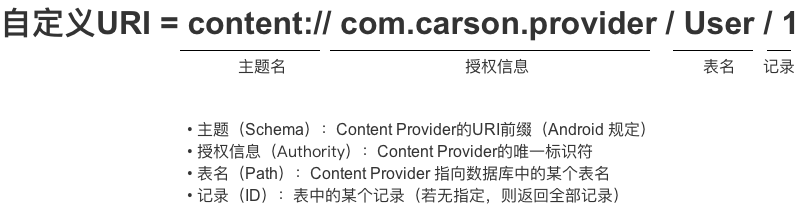
\includegraphics[width=.9\linewidth]{./pic/uri.png}
\begin{minted}[frame=lines,fontsize=\scriptsize,linenos=false]{java}
Uri uri = Uri.parse("content://com.carson.provider/User/1") // 设置URI
// 上述URI指向的资源是:名为 `com.carson.provider`的`ContentProvider` 中表名 为`User` 中的 `id`为1的数据

// 特别注意:URI模式存在匹配通配符: * # (两个)
//  *:匹配任意长度的任何有效字符的字符串
//     以下的URI 表示 匹配provider的任何内容
//     content://com.example.app.provider/* 
// #:匹配任意长度的数字字符的字符串
//     以下的URI 表示 匹配provider中的table表的所有行
//     content://com.example.app.provider/table/#
\end{minted}
\begin{itemize}
\item uri 的各个部分在安卓中都是可以通过代码获取的,下面我们就以下面这个 uri 为例来说下获取各个部分的方法:
\item \url{http://www.baidu.com:8080/wenku/jiatiao.html?id=123456&name=jack}
\end{itemize}
\begin{minted}[frame=lines,fontsize=\scriptsize,linenos=false]{java}
getScheme() // 获取 Uri 中的 scheme 字符串部分,在这里是 http
getHost()   // 获取 Authority 中的 Host 字符串,即 www.baidu.com
getPost()   // 获取 Authority 中的 Port 字符串,即 8080
getPath()   // 获取 Uri 中 path 部分,即 wenku/jiatiao.html
getQuery()  // 获取 Uri 中的 query 部分,即 id=15&name=du
\end{minted}

\subsection{MIME数据类型}
\label{sec-1-2}
\begin{itemize}
\item 作用:指定某个扩展名的文件用某种应用程序来打开
\begin{itemize}
\item 如指定.html文件采用text应用程序打开、指定.pdf文件采用flash应用程序打开
\end{itemize}
\end{itemize}

\subsubsection{ContentProvider根据 URI 返回MIME类型}
\label{sec-1-2-1}
\begin{minted}[frame=lines,fontsize=\scriptsize,linenos=false]{java}
ContentProvider.geType(uri) ;
\end{minted}
\subsubsection{MIME类型组成}
\label{sec-1-2-2}
\begin{itemize}
\item 每种MIME类型 由2部分组成 = 类型 + 子类型
\item MIME类型是 一个 包含2部分的字符串
\end{itemize}
\begin{minted}[frame=lines,fontsize=\scriptsize,linenos=false]{xml}
text / html
// 类型 = text、子类型 = html
text/css
text/xml
application/pdf
\end{minted}

\subsubsection{MIME类型形式}
\label{sec-1-2-3}
\begin{itemize}
\item MIME类型有2种形式:单条记录, 或是多条记录
\begin{minted}[frame=lines,fontsize=\scriptsize,linenos=false]{java}
// 形式1:单条记录  
vnd.android.cursor.item/自定义
// 形式2:多条记录(集合)
vnd.android.cursor.dir/自定义 

// 注:
  // 1. vnd:表示父类型和子类型具有非标准的、特定的形式。
  // 2. 父类型已固定好(即不能更改),只能区别是单条还是多条记录
  // 3. 子类型可自定义
\end{minted}
\item 实例说明
\end{itemize}
\begin{minted}[frame=lines,fontsize=\scriptsize,linenos=false]{xml}
<-- 单条记录 -->
  // 单个记录的MIME类型
  vnd.android.cursor.item/vnd.yourcompanyname.contenttype 

  // 若一个Uri如下
  content://com.example.transportationprovider/trains/122   
  // 则ContentProvider会通过ContentProvider.geType(url)返回以下MIME类型
  vnd.android.cursor.item/vnd.example.rail

<-- 多条记录 -->
  // 多个记录的MIME类型
  vnd.android.cursor.dir/vnd.yourcompanyname.contenttype 
  // 若一个Uri如下
  content://com.example.transportationprovider/trains 
  // 则ContentProvider会通过ContentProvider.geType(url)返回以下MIME类型
  vnd.android.cursor.dir/vnd.example.rail
\end{minted}

\subsection{ContentProvider类}
\label{sec-1-3}
\subsubsection{组织数据方式}
\label{sec-1-3-1}
\begin{itemize}
\item ContentProvider主要以 表格的形式 组织数据
\begin{itemize}
\item 同时也支持文件数据,只是表格形式用得比较多
\item 每个表格中包含多张表,每张表包含行 \& 列,分别对应记录 \& 字段,同数据库
\end{itemize}
\end{itemize}
\subsubsection{主要方法}
\label{sec-1-3-2}
\begin{itemize}
\item 进程间共享数据的本质是:添加、删除、获取 \& 修改(更新)数据(CRUD: create / read / update / delete)
\item 所以ContentProvider的核心方法也主要是上述几个作用
\end{itemize}
\begin{minted}[frame=lines,fontsize=\scriptsize,linenos=false]{java}
  // 外部进程向 ContentProvider 中添加数据
  public Uri insert(Uri uri, ContentValues values) 

  // 外部进程 删除 ContentProvider 中的数据
  public int delete(Uri uri, String selection, String[] selectionArgs) 

  // 外部进程更新 ContentProvider 中的数据
  public int update(Uri uri, ContentValues values, String selection, String[] selectionArgs)

  // 外部应用 获取 ContentProvider 中的数据
  public Cursor query(Uri uri, String[] projection, String selection, String[] selectionArgs,  String sortOrder)  

// 注:
  // 1. 上述4个方法由外部进程回调,并运行在ContentProvider进程的Binder线程池中(不是主线程)
  // 2. 存在多线程并发访问,需要实现线程同步
    // a. 若ContentProvider的数据存储方式是使用SQLite & 并且只有一个,则不需要,因为SQLite内部实现好了线程同步,若是多个SQLite则需要,因为SQL对象之间无法进行线程同步
    // b. 若ContentProvider的数据存储方式是内存,则需要自己实现线程同步

// 2个其他方法 -->
// ContentProvider创建后 或 打开系统后其它进程第一次访问该ContentProvider时 由系统进行调用
public boolean onCreate() 
// 注:运行在ContentProvider进程的主线程,故不能做耗时操作

// 得到数据类型,即返回当前 Url 所代表数据的MIME类型
public String getType(Uri uri)
\end{minted}

\begin{itemize}
\item Android为常见的数据(如通讯录、日程表等)提供了内置了默认的ContentProvider
\item 但也可根据需求自定义ContentProvider,但上述6个方法必须重写
\item 数据访问的方法 insert,delete 和 update 可能被多个线程同时调用,此时必须是线程安全的。(前面提到过)
\item 如果操作的数据属于集合类型,那么 MIME 类型字符串应该以 \uline{vnd.android.cursor.dir/} 开头,
\begin{itemize}
\item 要得到所有 tablename 记录: Uri 为 content://com.wang.provider.myprovider/tablename,那么返回的MIME类型字符串应该为:vnd.android.cursor.dir/table。
\end{itemize}
\item 如果要操作的数据属于非集合类型数据,那么 MIME 类型字符串应该以 \uline{vnd.android.cursor.item/} 开头,
\begin{itemize}
\item 要得到 id 为 10 的 tablename 记录,Uri 为 content://com.wang.provider.myprovider/tablename/10,那么返回的 MIME 类型字符串为:vnd.android.cursor.item/tablename 。
\end{itemize}

\item ContentProvider类并不会直接与外部进程交互,而是通过ContentResolver 类
\end{itemize}
\subsection{ContentResolver类}
\label{sec-1-4}
\begin{itemize}
\item 统一管理不同 ContentProvider间的操作
\begin{itemize}
\item 即通过 URI 即可操作 不同的ContentProvider 中的数据
\item 外部进程通过 ContentResolver类 从而与ContentProvider类进行交互
\end{itemize}
\item 为什么要使用通过ContentResolver类从而与ContentProvider类进行交互,而不直接访问ContentProvider类?
\begin{itemize}
\item 一般来说,一款应用要使用多个ContentProvider,若需要了解每个ContentProvider的不同实现从而再完成数据交互,操作成本高 \& 难度大
\item 所以再ContentProvider类上加多了一个 ContentResolver类对所有的ContentProvider进行统一管理。
\end{itemize}
\item ContentResolver 类提供了与ContentProvider类相同名字 \& 作用的4个方法
\end{itemize}
\begin{minted}[frame=lines,fontsize=\scriptsize,linenos=false]{java}
// 外部进程向 ContentProvider 中添加数据
public Uri insert(Uri uri, ContentValues values)  

// 外部进程 删除 ContentProvider 中的数据
public int delete(Uri uri, String selection, String[] selectionArgs)

// 外部进程更新 ContentProvider 中的数据
public int update(Uri uri, ContentValues values, String selection, String[] selectionArgs)  

// 外部应用 获取 ContentProvider 中的数据
public Cursor query(Uri uri, String[] projection, String selection, String[] selectionArgs, String sortOrder)
\end{minted}
\begin{itemize}
\item 实例说明
\end{itemize}
\begin{minted}[frame=lines,fontsize=\scriptsize,linenos=false]{java}
// 使用ContentResolver前,需要先获取ContentResolver
// 可通过在所有继承Context的类中 通过调用getContentResolver()来获得ContentResolver
ContentResolver resolver =  getContentResolver(); 

// 设置ContentProvider的URI
Uri uri = Uri.parse("content://cn.scu.myprovider/user"); 
 
// 根据URI 操作 ContentProvider中的数据
// 此处是获取ContentProvider中 user表的所有记录 
Cursor cursor = resolver.query(uri, null, null, null, "userid desc");
\end{minted}
\begin{itemize}
\item Android 提供了3个用于辅助ContentProvider的工具类:
\begin{itemize}
\item ContentUris
\item UriMatcher
\item ContentObserver
\end{itemize}
\end{itemize}
\subsection{ContentUris类}
\label{sec-1-5}
\begin{itemize}
\item 作用:操作 URI
\item 核心方法有两个:withAppendedId() \&parseId()
\end{itemize}
\begin{minted}[frame=lines,fontsize=\scriptsize,linenos=false]{java}
// withAppendedId()作用:向URI追加一个id
Uri uri = Uri.parse("content://cn.scu.myprovider/user") 
Uri resultUri = ContentUris.withAppendedId(uri, 7);  
// 最终生成后的Uri为:content://cn.scu.myprovider/user/7

// parseId()作用:从URL中获取ID
Uri uri = Uri.parse("content://cn.scu.myprovider/user/7") 
long personid = ContentUris.parseId(uri); 
//获取的结果为:7
\end{minted}
\subsection{UriMatcher类}
\label{sec-1-6}
\begin{itemize}
\item 在ContentProvider 中注册URI
\item 根据 URI 匹配 ContentProvider 中对应的数据表
\end{itemize}
\begin{minted}[frame=lines,fontsize=\scriptsize,linenos=false]{java}
// 步骤1:初始化UriMatcher对象
    UriMatcher matcher = new UriMatcher(UriMatcher.NO_MATCH); 
    // 常量UriMatcher.NO_MATCH = 不匹配任何路径的返回码
    // 即初始化时不匹配任何东西

// 步骤2:在ContentProvider 中注册URI(addURI())
    int URI_CODE_a = 1;
    int URI_CODE_b = 2;
    matcher.addURI("cn.scu.myprovider", "user1", URI_CODE_a); 
    matcher.addURI("cn.scu.myprovider", "user2", URI_CODE_b); 
    // 若URI资源路径 = content://cn.scu.myprovider/user1 ,则返回注册码URI_CODE_a
    // 若URI资源路径 = content://cn.scu.myprovider/user2 ,则返回注册码URI_CODE_b

    //如果match()方法匹配content://com.wang.provider.myprovider/tablename/11路径,返回匹配码为2
    matcher.addURI("com.wang.provider.myprovider", "tablename/#", 2);

// 步骤3:根据URI 匹配 URI_CODE,从而匹配ContentProvider中相应的资源(match())
@Override public String getType(Uri uri) {   
      Uri uri = Uri.parse(" content://cn.scu.myprovider/user1");   

      switch(matcher.match(uri)) {   
      // 根据URI匹配的返回码是URI_CODE_a
      // 即matcher.match(uri) == URI_CODE_a
      case URI_CODE_a:   
          // 如果根据URI匹配的返回码是URI_CODE_a,则返回ContentProvider中的名为tableNameUser1的表
          return tableNameUser1;   
      case URI_CODE_b:   
          // 如果根据URI匹配的返回码是URI_CODE_b,则返回ContentProvider中的名为tableNameUser2的表
          return tableNameUser2;
    }   
}
\end{minted}
\begin{itemize}
\item 注意,添加第三个个 URI 时,路径后面的 id 采用了通配符形式 “\#”,表示只要前面三个部分都匹配上了就 OK。
\item 第三步,注册完需要匹配的 Uri 后,可以使用 matcher.match(Uri) 方法对输入的 Uri 进行匹配,如果匹配就返回对应的匹配码,匹配码为调用 addURI() 方法时传入的第三个参数。
\end{itemize}
\subsection{ContentObserver类}
\label{sec-1-7}
\begin{itemize}
\item 定义:内容观察者
\item 作用:观察 Uri引起 ContentProvider 中的数据变化 \& 通知外界(即访问该数据访问者)
\begin{itemize}
\item 当ContentProvider 中的数据发生变化(增、删 \& 改)时,就会触发该 ContentObserver类
\end{itemize}
\end{itemize}
\begin{minted}[frame=lines,fontsize=\scriptsize,linenos=false]{java}
// 步骤1:注册内容观察者ContentObserver
// 通过ContentResolver类进行注册,并指定需要观察的URI
getContentResolver().registerContentObserver(uri);

// 步骤2:当该URI的ContentProvider数据发生变化时,通知外界(即访问该ContentProvider数据的访问者)
public class UserContentProvider extends ContentProvider { 
    public Uri insert(Uri uri, ContentValues values) { 
        db.insert("user", "userid", values); 
        // 通知访问者
        getContext().getContentResolver().notifyChange(uri, null); 
    } 
}
// 步骤3:解除观察者
getContentResolver().unregisterContentObserver(uri);
// 同样需要通过ContentResolver类进行解除
\end{minted}
\begin{itemize}
\item 上面说得可能还不是太彻底,下面再重新写一下
\item 如果ContentProvider的访问者需要知道数据发生的变化,可以在ContentProvider发生数据变化时调用getContentResolver().notifyChange(uri, null)来通知注册在此URI上的访问者。只给出类中监听部分的代码:
\end{itemize}
\begin{minted}[frame=lines,fontsize=\scriptsize,linenos=false]{java}
public class MyProvider extends ContentProvider {
   public Uri insert(Uri uri, ContentValues values) {
      db.insert("tablename", "tablenameid", values);
      getContext().getContentResolver().notifyChange(uri, null);
   }
}
\end{minted}
\begin{itemize}
\item 而访问者必须使用 ContentObserver 对数据(数据采用 uri 描述)进行监听,当监听到数据变化通知时,系统就会调用 ContentObserver 的 onChange() 方法:
\end{itemize}
\begin{minted}[frame=lines,fontsize=\scriptsize,linenos=false]{java}
getContentResolver().registerContentObserver(Uri.parse("content://com.ljq.providers.personprovider/person"),
       true, new PersonObserver(new Handler()));
public class PersonObserver extends ContentObserver{
   public PersonObserver(Handler handler) {
      super(handler);
   }
   public void onChange(boolean selfChange) {
      //to do something
   }
}
\end{minted}
\subsection{优点}
\label{sec-1-8}
\subsubsection{安全}
\label{sec-1-8-1}
\begin{itemize}
\item ContentProvider为应用间的数据交互提供了一个安全的环境:允许把自己的应用数据根据需求开放给 其他应用 进行 增、删、改、查,而不用担心因为直接开放数据库权限而带来的安全问题
\end{itemize}
\subsubsection{访问简单 \& 高效}
\label{sec-1-8-2}
\begin{itemize}
\item 对比于其他对外共享数据的方式,数据访问方式会因数据存储的方式而不同:
\begin{itemize}
\item 采用 文件方式 对外共享数据,需要进行文件操作读写数据;
\item 采用 Sharedpreferences 共享数据,需要使用sharedpreferences API读写数据,这使得访问数据变得复杂 \& 难度大。
\item 而采用ContentProvider方式,其 解耦了 底层数据的存储方式,使得无论底层数据存储采用何种方式,外界对数据的访问方式都是统一的,这使得访问简单 \& 高效
\item 如一开始数据存储方式 采用 SQLite 数据库,后来把数据库换成 MongoDB,也不会对上层数据ContentProvider使用代码产生影响
\end{itemize}
\end{itemize}
% Emacs 27.1 (Org mode 8.2.7c)
\end{document}